% IMPORTANT NOTE: This is a slightly adapted Copy of https://tex.stackexchange.com/questions/181081/clickable-chapters-on-the-right-side-of-each-page
% The credit goes to Gonzalo Medina, I only made slight changes (Converted to landscape and made Tabs nameable)

% ANOTHER IMPORTANT NOTE: The Boxlayout with Titles was copied from here: https://www.overleaf.com/articles/130-cheat-sheet/ntwtkmpxmgrp
% The Credit goes to Drew Ulick

\documentclass[8pt]{article}
% Article
% \documentclass[9pt]{extarticle}
\usepackage[landscape, left=0.75cm, top=1cm, right=0.75cm, bottom=1.5cm, footskip=15pt]{geometry}
\usepackage{background}
\usepackage{etoolbox}
\usepackage{graphicx}
\usepackage{totcount}
\usepackage{lipsum}
\usepackage{hyperref}
\usepackage{amsmath}
\usepackage{amssymb}

% Mathematical typesetting & symbols
\usepackage{amsthm, mathtools, amssymb} 
\usepackage{marvosym, wasysym}
\allowdisplaybreaks

% Math helper stuff
\def\limn{\lim_{n\to \infty}}
\def\limxo{\lim_{x\to 0}}
\def\limxi{\lim_{x\to\infty}}
\def\limxn{\lim_{x\to-\infty}}
\def\sumk{\sum_{k=1}^\infty}
\def\sumn{\sum_{n=0}^\infty}
\def\R{\mathbf{R}}
\def\dx{\text{ d}x}

% color text
\usepackage{xcolor}

% Tables
\usepackage{tabularx, multirow}
\usepackage{booktabs}
\renewcommand*{\arraystretch}{2}

% image directory
\graphicspath{ {./assets/} }

% For accessing arrays
\usepackage{etoolbox}

% for emumerating
\usepackage{enumerate}

% for color coding
\usetikzlibrary{backgrounds}

% for light font +C
\usepackage{color}
\definecolor{light}{rgb}{0.5, 0.5, 0.5}
\def\light#1{{\color{light}#1}}



% for multicolumn
\usepackage{multicol}
\usepackage{multirow}

% to have access to the total number of sections
\regtotcounter{section}

% the main part; as background material we place the border, 
% the section (current and other) tabs and the page number
\backgroundsetup{
scale=1,
color=black,
angle=0,
opacity=1,
contents={}
}

\usepackage{sectsty}
\subsectionfont{\normalfont\small\bfseries\underline}
\subsubsectionfont{\normalfont\small}
\begin{document}

\setlength{\columnseprule}{0.4pt}
\pagenumbering{arabic}
\begin{multicols*}{3}

\section{Folgen}
\hypertarget{sec:0}{}

% Konvergenz

  \subsection {Konvergenz}

Die Folge $(a_n)_{n \geq 1}$ \textbf{konvergiert} gegen $a$ für
$n \rightarrow \infty$, falls gilt:
\begin{align*}
  \forall \epsilon > 0 \; \exists n_0 = n_0(\epsilon) \in \mathbf{N} \; \forall n \geq n_0 : |a_n - a| < \epsilon
\end{align*}
Wir schreiben dann:
\begin{align*}
  a = \lim_{n \rightarrow \infty} a_n \text{ oder }a_n \rightarrow a \; (n \rightarrow \infty)
\end{align*}
und nennen $a$ den \textbf{Grendwert/ Limes} der Folge $(a_n)_{n \geq 1}$.
Existiert der Limes nicht, so heisst die Folge \textbf{divergent}. Zu bemerken ist:
\begin{align*}
  (a_n)_{n \geq 1} \text{ konvergent } \Rightarrow (a_n)_{n \geq 1} \text{ beschränkt }
\end{align*}
% Monotone Konvergenz
  \subsection{Monotone Konvergenz}
Sei die Folge $(a_n)_{n \geq 1}$ monoton wachsend und nach oben beschränkt.
Dann konvergiert $(a_n)_{n \geq 1}$ mit Grenzwert:
\begin{align*}
  \lim_{n \rightarrow \infty} a_n = \text{sup} \{a_n : n \geq 1\}
\end{align*}
Ist die Folge $(a_n)_{n \geq 1}$ monoton fallend und nach unten beschränkt,
so konvergiert $(a_n)_{n \geq 1}$ mit Grenzwert:
\begin{align*}
  \lim_{n \rightarrow \infty} a_n = \text{inf} \{a_n : n \geq 1\}
\end{align*}
% Cauchy Kriterium
\subsection{Cauchy Kriterium}

Die Folge $(a_n)_{n \geq 1}$ ist genau dann konvergent, falls:
$$
  \forall \epsilon > 0 \; \exists N \geq 1 \text{ so dass } |a_n - a_m| < \epsilon \; \; \forall n, m \geq N\\
$$
% Rechnen mit Limes

  \subsection {Rechnen mit Limes}

Seien die Folgen $(a_n)_{n \geq 1}$, $(b_n)_{n \geq 1}$ konvergent mit
$\lim_{n \rightarrow \infty} a_n = a$ und $\lim_{n \rightarrow \infty} b_n = b$.
Dann gilt:
\begin{enumerate}[(i)]
  \item $\lim_{n \rightarrow \infty} (a_n + b_n) = \lim_{n \rightarrow \infty} a_n + \lim_{n \rightarrow \infty} b_n$
  \item $\lim_{n \rightarrow \infty} (a_n * b_n) = \lim_{n \rightarrow \infty} a_n * \lim_{n \rightarrow \infty} b_n$
  \item Falls zusätzlich $b_n \neq 0 \; \forall n \geq 1$ und $b \neq 0$ gegeben ist, so gilt: $\lim_{n \rightarrow \infty} (a_n / b_n) = a / b$.
  \item Falls es ein $K \geq 1$ gibt mit $a_n \leq b_n \; \forall n \geq K$, dann folgt $a \leq b$.
\end{enumerate}
% Limes Superior/ Inferior
  \subsection{Limes Superior/ Inferior}
Sei eine Folge $(a_n)_{n \geq 1}$ beschränkt. Wir können dann zwei monotone
Folgen $(b_n)_{n \geq 1}$ und $(c_n)_{n \geq 1}$ definieren, welche dann einen Grenzwert besitzen.
Sei für jedes $n \geq 1$:
\begin{gather*}
  b_n = \inf\{a_k : k \geq n\} \text{ und } c_n = \sup\{a_k : k \geq n\}\\
  b_n \leq b_{n + 1}\\
  c_{n + 1} \leq c_n
\end{gather*}
Da also beide Folgen beschränkt sind und konvergieren, können wir aufgrund von
Monotoner Konvergenz folgern:
\begin{gather*}
  \liminf_{n \rightarrow \infty} a_n := \lim_{n \rightarrow \infty} b_n\\
  \limsup_{n \rightarrow \infty} a_n := \lim_{n \rightarrow \infty} c_n\\
  \liminf_{n \rightarrow \infty} a_n \leq \limsup_{n \rightarrow \infty} a_n
\end{gather*}
Es gilt auch, dass $(a_n)_{n \geq 1}$ genau dann konvergiert, falls $(a_n)_{n \geq 1}$
beschränkt ist und $\liminf_{n \rightarrow \infty} a_n = \limsup_{n \rightarrow \infty} a_n$
% Bolzano-Weierstrass
 \subsection{Bolzano-Weierstrass}
Jede beschränkte Folge besitzt eine konvergente Teilfolge.
% Sandwichsatz für Folgen
  \subsection {Sandwichsatz für Folgen}
Seien $(a_n)_{n \geq 1}$ und $(b_n)_{n \geq 1}$ konvergente Folgen mit demselben Limes
$\alpha \in \mathbf{R}$. Ist $K \in \mathbf{N}$ und $(c_n)_{n \geq 1}$ eine Folge
mit der Eigenschaft: $$a_n \leq c_n \leq b_n \; \; \; \forall n \geq K$$ so konvergiert
auch $(c_n)_{n \geq 1}$ gegen $\alpha$.
% Limes Binom Trick
  \subsection{Limes Binom Trick}
Gegeben die Summe zweier Wurzeln könnte man wie folgt
vorgehen (Bsp.):
$$
  \lim_{x \rightarrow \infty} (\sqrt{x + 5} - \sqrt{x - 3}) = \lim_{x \rightarrow \infty} (\frac{(x + 5) - (x - 3)}{\sqrt{x + 5} + \sqrt{x - 3}})
$$
% Limes Substitution Trick
  \subsection{Limes Substitution Trick}
Hier ein Beispiel:
$$
  \lim_{x \rightarrow \infty} x^2 (1 - cos(\frac{1}{x}))
$$\\
Substitutiere nun $u = \frac{1}{x}$:
$$
\lim_{u \rightarrow 0} \frac{1 - cos(u)}{u^2} = \lim_{u \rightarrow 0} \frac{sin(u)}{2u} = \lim_{u \rightarrow 0} \frac{cos(u)}{2} = \frac{1}{2}
$$
% Limes Taylor Trick

  \subsection{Limes Taylor Trick}

Mithilfe der Reihenentwicklung von $e^x$ und $sin(x)$:
$$
\lim_{n \rightarrow \infty} \frac{e^{1/n} - 1 - \frac{1}{n}}{1 - n * sin(\frac{1}{n})} = \frac{\frac{1}{2}n^{-2} + \mathcal{O}(n^{-3})}{1 - n(n^{-1} - \frac{1}{6}n^{-3} + \mathcal{O}(n^{-5}))} = 3
$$

% Rekurrenz Beispiel
  \subsection {Rekurrenz Beispiel}
Die folgenden Schritte solten bei der Auflösung einer Rekursiven Folge in betracht gezogen werden:
\begin{enumerate}
  \item Zeige Monotonie (Durch Induktion)
  \item Zeige Obere oder Untere Schranke (Evt. Induktion)
  \item Verwende $\lim_{n \rightarrow \infty} a_n = \lim_{n \rightarrow \infty} a_{n + 1}$ (Da für jede Teilfolge der gleiche Grenzwert gilt)
\end{enumerate}
% Punktweise Konvergenz
 \subsection{Punktweise Konvergenz}
Die Funktionenfolge $(f_n)_{n \geq 0}$ konvergiert punktweise gegen eine Funktion
$f:\mathbf{D} \rightarrow \mathbf{R}$ falls für alle $x \in \mathbf{D}$, $f(x) = \lim_{n \rightarrow \infty} f_n(x)$ gilt. Konkret:
\begin{align*}
  &\forall x \in \mathbf{D} \;\;\; \forall \epsilon > 0 \;\;\; \exists N_{x, \epsilon} \geq 1 \text{ so dass }\\
  &\forall n \geq N \;\;\; |f_n(x) - f(x)| < \epsilon
\end{align*}
% Gleichmässige Konvergenz
 \subsection{Gleichmässige Konvergenz}
Die Funktionenfolge $(f_n)_{n \geq 0}$ konvergiert gleichmässig in $\mathbf{D}$ gegen eine Funktion
$f:\mathbf{D} \rightarrow \mathbf{R}$ falls für alle $x \in \mathbf{D}$, $f(x) = \lim_{n \rightarrow \infty} f_n(x)$ gilt. Konkret:
\begin{align*}
  &\forall \epsilon > 0 \;\;\; \exists N_{\epsilon} \geq 1 \text{ so dass }\\
  &\forall n \geq N \;\;\;\forall x \in \mathbf{D} \;\;\; |f_n(x) - f(x)| < \epsilon
\end{align*}
Weiter ist folgenes Kriterium äquivalent:
\begin{align*}
  &\forall \epsilon > 0 \;\;\; \exists N \geq 1 \text{ so dass }\\
  &\forall n, m \geq N \;\;\;\forall x \in \mathbf{D} \;\;\; |f_n(x) - f_m(x)| < \epsilon
\end{align*}
Konvergiert eine Funktionenfolge $(f_n)_{n \geq 1}, f_n:\mathbf{D} \subset \mathbf{R} \rightarrow \mathbf{R}$
bestehend aus in $\mathbf{D}$ stetigen Funktionen gleichmässig gegen die Funktion $f:\mathbf{D} \rightarrow \mathbf{R}$, so
ist $f$ in $\mathbf{D}$ \textbf{stetig}.\\
\\
\textbf{Beispiel:}
$f_n : \mathbf{R} \rightarrow \mathbf{R}, f_n(x) = \sqrt{|x| + \frac{1}{n^3}}$
Wie lautet der punktweise Limes der Funktionsfolge $f_n$? Konvergiert $f_n$ gleichmässig auf  $\mathbf{R}$?\\
\textbf{Punktweise Konvergenz:} Wir fixieren $x \in R$ und bilden den Limes für $n \rightarrow \infty$

$\lim_{n \to \infty} f_n(x) = \lim_{n \rightarrow \infty} \sqrt{|x| + \frac{1}{n^3}} = \sqrt{|x|} = f(x)$\\
Die Funktionenfolge konvergiert somit punktweise gegen den punktweisen Grenzwert $f(x) = \sqrt{|x|}$\\
\textbf{Gleichmässige Konvergenz:} Wir müssen zeigen, dass $\lim_{n \to \infty} sup_{x \in \mathbf{R}} |f_n(x) - f(x)| = 0$ gilt. Wir berechnen also zuerst den Ausdruck $sup_{x \in \mathbf{R}} |f_n(x) - f(x)|$
\begin{align*}
	&sup_{x \in \mathbf{R}} |f_n(x) - f(x)| = sup_{x \in \mathbf{R}} |\sqrt{|x| + \frac{1}{n^3}} - \sqrt{|x|}|\\
	& =  sup_{x \in \mathbf{R}} |(\sqrt{|x| + \frac{1}{n^3}} - \sqrt{|x|}) \frac{(\sqrt{|x| + \frac{1}{n^3}} + \sqrt{|x|})}{(\sqrt{|x| + \frac{1}{n^3}} + \sqrt{|x|)}}| \\
	& = sup_{x \in \mathbf{R}} |\frac{\frac{1}{n^3}}{\sqrt{|x| + \frac{1}{n^3}} + \sqrt{|x|}}|
\end{align*}

Da $|x|$ positiv ist, wird das Supremum von $|\frac{\frac{1}{n^3}}{\sqrt{|x| + \frac{1}{n^3}} + \sqrt{|x|}}|$ bei $x = 0$ angenommen. Es gilt somit

\begin{align*}
	& sup_{x \in \mathbf{R}} |f_n(x) - f(x)| = sup_{x \in \mathbf{R}} |\frac{\frac{1}{n^3}}{\sqrt{|x| + \frac{1}{n^3}} + \sqrt{|x|}}|\\
 	&= \frac{\frac{1}{n^3}}{\sqrt{\frac{1}{n^3}}} = \frac{1}{n^{\frac{3}{2}}}
\end{align*}
Somit konvergiert die Funktionenfolge $f_n$ auf $\mathbf{R}$ gleichmässig gegen $f$.




% Grenzwerte von Funktionen
  \subsection {Grenzwerte von Funktionen}
Sei $f:\mathbf{D} \rightarrow \mathbf{R}$, $x_0 \in \mathbf{R}$ ein Häufungspunkt von $\mathbf{D}$.
Dann ist $A \in \mathbf{R}$ der Grenzwert von $f(x)$ für $x \rightarrow x_0$, bezeichnet mit
$$
  \lim_{x \rightarrow x_0} f(x) = A
$$
falls $\forall \epsilon > 0 \;\;\; \exists \delta > 0$ so dass
$$
  \forall x \in \mathbf{D} \cap (]x_0-\delta, x_0 + \delta[ \setminus \{x_0\}) : |f(x) - A| < \epsilon
$$
% Rechnen mit Limes Für Funktionen
\subsection{Rechnen mit Limes Für Funktionen}
Seien die Funktionen $f, g: \mathbf{D} \rightarrow \mathbf{R}$ konvergent mit
$\lim_{x \rightarrow x_0} f(x) = A$ und $\lim_{x \rightarrow x_0} g(x) = B$. Sei weiter
$x_0 \in \mathbf{R}$ ein Häufungspunkt von $\mathbf{D}$.
Dann gilt:
\begin{enumerate}[(i)]
  \item $\lim_{x \rightarrow x_0} (f + g)(x) = \lim_{x \rightarrow x_0} f(x) + \lim_{x \rightarrow x_0} g(x)$
  \item $\lim_{x \rightarrow x_0} (f * g)(x) = \lim_{x \rightarrow x_0} f(x) * \lim_{x \rightarrow x_0} g(x)$
  \item Sei $f, g: \mathbf{D} \rightarrow \mathbf{R} \text{ mit } f \leq g$. Dann folgt:
  $$
    \lim_{x \rightarrow x_0} f(x) \leq \lim_{x \rightarrow x_0} g(x)
  $$
  falls beide Grenzwerte existieren.
  \item Seien $\mathbf{D}, \mathbf{E} \subset \mathbf{R}$ und $f: \mathbf{D} \rightarrow \mathbf{E}$ eine Funktion. Wir nehmen an, dass $$y_0 := \lim_{x \rightarrow x_0} f(x)$$ existiert
  und $y_0 \in \mathbf{E}$. Falls $g:\mathbf{E} \rightarrow \mathbf{R}$ stetig in $y_0$ folgt:
  $$\lim_{x \rightarrow x_0} g(f(x)) = g(y_0)$$
\end{enumerate}
% Sandwichsatz für Funktionen
  \subsection{Sandwichsatz für Funktionen}
Falls $g_1 \leq f \leq g_2$ und
  $$
  \lim_{x \rightarrow x_0} g_1(x) = \lim_{x \rightarrow x_0} g_2(x)
  $$
  dann existiert $\lim_{x \rightarrow x_0} f(x)$ und
  $$
  \lim_{x \rightarrow x_0} f(x) = \lim_{x \rightarrow x_0} g_1(x)
  $$
% Links- und Rechtsseitige Grenzwerte
 \subsection{Links- und Rechtsseitige Grenzwerte}
Sei $f: \mathbf{D} \rightarrow \mathbf{R}$, $x_0 \in \mathbf{R}$. Wir nehmen an, dass
$x_0$ ein Häufungspunkt von $\mathbf{D} \;\cap\; ]x_0, +\infty[$ ist. Falls der Grenzwert
der Eingeschränkten Funktionen $f$ im Bereich $\mathbf{D} \;\cap\; [x_0, +\infty[$ für
$x \rightarrow x_0$ existiert, wird er mit $\lim_{x \rightarrow x_0^+} f(x)$ bezeichnet und
nennt sich \textbf{rechtsseitiger Grenzwert} von $f$ bei $x_0$.\\
Der \textbf{linksseitige Grenzwert} ist analog definiert für den Bereich $\mathbf{D} \;\cap\; ]-\infty, x_0]$
für $x \rightarrow x_0$, falls er existiert. Es wird mit $\lim_{x \rightarrow x_0^-} f(x)$ bezeichnet.\\
Besitzt die Funktion $f(x)$ an der Stelle $x_0$ den Grenzwert $L$, so gilt:
$$
  \lim_{x \rightarrow x_0+} f(x) = \lim_{x \rightarrow x_0-} f(x) = \lim_{x \rightarrow x_0} f(x) = L
$$
\section{Reihen}
\hypertarget{sec:1}{}
% Konvergenz
  \subsection{Konvergenz}
Die Reihe $\sum_{k = 1}^{\infty} a_k$ ist konvergent, falls die Folge der
Partialsummen $(S_n)_{n \geq 1} = \sum_{k = 1}^{n} a_k$
konvergiert. In diesem Fall definieren wir:
\begin{align*}
  \sum_{k = 1}^{\infty} a_k := \lim_{n \rightarrow \infty} S_n
\end{align*}\\
% Monotone Konvergenz
  \subsection {Monotone Konvergenz}
Sei $\sum_{k = 1}^\infty a_k$ eine Reihe mit $a_k \geq 0 \;\; \forall k \in \mathbf{N}$.
Die Reihe konvergiert genau dann, wenn die Folge der Parialsummen $(S_n)_{n \geq 1}$ nach
oben beschränkt ist.
% Cauchy Kriterium
\subsection{Cauchy Kriterium}
Die Reihe $\sum_{k = 1}^{\infty} a_k$ ist geau dann konvergent, falls:
$$
  \forall \epsilon > 0 \; \exists N \geq 1 \text{ mit } \left| \sum_{k = n}^m a_k \right| < \epsilon \; \; \; \forall m \geq n \geq N
$$
% Rechnen mit Konvergenten Reihen
\subsection{Rechnen mit Konvergenten Reihen}
Seien $\sum_{k = 1}^\infty a_k$ und $\sum_{k = 1}^\infty b_k$ konvergent, sowie $\alpha \in \mathbf{C}$.
Dann gilt:
\begin{enumerate}[(i)]
  \item $\sum_{k = 1}^\infty (a_k + b_k)$ ist konvergent und $\sum_{k = 1}^\infty (a_k + b_k) = \sum_{k = 1}^\infty a_k + \sum_{k = 1}^\infty b_k$
  \item $\sum_{k = 1}^\infty \alpha * a_k$ ist konvergent und $\sum_{k = 1}^\infty \alpha * a_k = \alpha * \sum_{k = 1}^\infty a_k$
\end{enumerate}
Konvergieren die Reihen $\sum_{i = 0}^\infty a_i$ und $\sum_{j = 0}^\infty b_j$ absolut,
so gilt zusätzlich für das Cauchy Produkt:
\begin{enumerate}[(iii)]
  \item $\sum_{n = 0}^\infty (\sum_{j = 0}^n a_{n - j} * b_j) = (\sum_{i = 0}^\infty a_i) * (\sum_{j = 0}^\infty b_j)$
\end{enumerate}
% Absolute Konvergenz
\subsection {Absolute Konvergenz}
Eine Reihe $\sum_{k = 1}^{\infty} a_k$ heisst \textbf{absolut konvergent},
falls $\sum_{k = 1}^{\infty} |a_k|$ konvergiert. Weiter sind \textbf{absolut konvergente Reihen
auch konvergent} und es gilt:
$$
  \left| \sum_{k = 1}^{\infty} a_k \right| \leq \sum_{k = 1}^{\infty} |a_k|
$$
% Reihen Umordnung

\subsection{Reihen Umordnung}

Konvergiert $\sum_{n = 1}^\infty a_n$ absolut, dann konvergiert auch jede Umordnung
der Reihe $a_n' = a_{\phi(n)}$ (wobei $\phi$ bijektiv) und hat denselben Grenzwert.

% Potenzreihe
\subsection {Potenzreihe}
Die Potenzreihe $\sum_{k = 0}^\infty c_k z^k$ konvergiert absolut für alle $z \in \mathbf{C}$
mit $|z| < \rho$ (divergiert bei $|z| > \rho$), wobei
$$
  \rho := \begin{cases}
    +\infty &\text{Falls} \limsup_{k \rightarrow \infty} \sqrt[k]{|c_k|} = 0\\
    \frac{1}{\limsup_{k \rightarrow \infty} \sqrt[k]{|c_k|}} &\text{Falls} \limsup_{k \rightarrow \infty} \sqrt[k]{|c_k|} > 0\\
  \end{cases}
$$
\begin{center}
  \color{red}
  \textbf{Ränder Prüfen!}
\end{center}
% Nullfolgenkriterium
\subsection{Nullfolgenkriterium}
$$
  \lim_{n \rightarrow \infty} |a_n| \neq 0 \Rightarrow \sum_{n = 0}^\infty a_n \text{ divergiert}
$$
% Wurzelkriterium

\subsection{Wurzelkriterium}

\begin{align*}
  \limsup_{n \rightarrow \infty} \sqrt[n]{|a_n|} < 1 &\Rightarrow \sum_{n = 1}^\infty a_n \text{ konvergiert absolut.}\\
  \limsup_{n \rightarrow \infty} \sqrt[n]{|a_n|} > 1 &\Rightarrow \sum_{n = 1}^\infty a_n \text{ und } \sum_{n = 1}^\infty |a_n| \text{ divergieren.}
\end{align*}
% Quotientenkriterium

\subsection{Quotientenkriterium}

Sei $(a_n)_{n \geq 1}$ eine Folge mit $a_n \neq 0$
\begin{align*}
  \limsup_{n \rightarrow \infty} \frac{|a_{n+1|}}{|a_n|} < 1 &\Rightarrow \sum_{n = 1}^\infty a_n \text{ konvergiert absolut.}\\
  \liminf_{n \rightarrow \infty} \frac{|a_{n+1|}}{|a_n|} > 1 &\Rightarrow \sum_{n = 1}^\infty a_n \text{ divergiert.}
\end{align*}
% Vergleichssatz

\subsection{Vergleichssatz}

Seien $\sum_{k = 1}^\infty a_k$ und $\sum_{k = 1}^\infty b_k$ Reihen mit:
\begin{align*}
  0 \leq a_k &\leq b_k \; \; \; \forall k \geq 1\\
  \sum_{k = 1}^\infty b_k \text{ konvergent} &\Rightarrow \sum_{k = 1}^\infty a_k \text{ konvergent}\\
  \sum_{k = 1}^\infty a_k \text{ divergent} &\Rightarrow \sum_{k = 1}^\infty b_k \text{ divergent}
\end{align*}
% Integraltest
\subsection{Integraltest}

Sei $f(x)$ eine stetige, positive und monoton fallende
Funktion auf $[k, \infty)$ und $f(n) = a_n$:
\begin{align*}
\int_{k}^{\infty} f(x) dx \text{ konvergiert} \Rightarrow \sum_{n = k}^{\infty} a_n \text{ konvergiert}\\
\int_{k}^{\infty} f(x) dx \text{ divergiert}  \Rightarrow \sum_{n = k}^{\infty} a_n \text{ divergiert}
\end{align*}
% Leibniz Kriterium

\subsection{Leibniz Kriterium}

Sei $(a_n)_{n \geq 1}$ monoton fallend mit $a_n \geq 0 \; \; \; \forall n \geq 1$ und
$\lim_{n \rightarrow \infty} a_n = 0$. Dann konvergiert
$$
  S := \sum_{k = 1}^\infty (-1)^{k + 1} a_k
$$
und es gilt: $a_1 - a_2 \leq S \leq a_1$
% Gleichmässige Konvergenz

\subsection{Gleichmässige Konvergenz}

Die Reihe $\sum_{k=0}^\infty f_k(x)$ konvergiert gleichmässig in $\mathbf{D}$ falls die durch
$$
  S_n(x) := \sum_{k=0}^n f_k(x)
$$
definierte Funktionenfolge gleichmässig konvergiert.\\
Gilt weiter, dass $f_n: \mathbf{D} \subset \mathbf{R} \rightarrow \mathbf{R}$ eine Folge
stetiger Funktionen ist und eine Folge $C_n$ existiert, so dass
\begin{align*}
  |f_n(x)| \leq C_n \;\;\; \forall x \in \mathbf{D}
\end{align*}
und dass $\sum_{n = 0}^\infty c_n$ konvergiert, dann konvergiert die Reihe
$\sum_{n = 0}^\infty f_n(k)$ gleichmässig in $\mathbf{D}$ und deren Grenzwert
\begin{align*}
  f(x) := \sum_{n = 0}^\infty f_n(k)
\end{align*}
ist eine in $\mathbf{D}$ stetige Funktion.
\section{Stetigkeit}
\hypertarget{sec:2}{}
% Stetigkeit einer Funktion in einem Punk

\subsection{Stetigkeit einer Funktion in einem Punk}

Sei $\mathbf{D} \subseteq \mathbf{R}$, $x_0 \in \mathbf{D}$. Die Funktion
$f: \mathbf{D} \rightarrow \mathbf{R}$ ist in $x_0$ \textbf{stetig}, falls
es für jedes $\epsilon > 0$ ein $\delta > 0$ gibt, so dass für alle $x \in \mathbf{D}$
gilt:
\begin{align*}
  |x - x_0| < \delta \Rightarrow |f(x) - f(x_0)| < \epsilon 
\end{align*}
Hier noch eine äquivalente Definition: Falls für jede Folge $(a_n)_{n \geq 1}$ mit
$\lim_{n \rightarrow \infty} a_n = x_0$ folgendes gilt:
\begin{align*}
  f(\lim_{n \rightarrow \infty} a_n) = f(x_0) = \lim_{n \rightarrow \infty} f(a_n)
\end{align*}
ist die Funktion $f$ in $x_0$ stetig.
% Stetigkeit einer Funktion

\subsection{Stetigkeit einer Funktion}

Die Funktion $f: \mathbf{D} \rightarrow \mathbf{R}$ ist \textbf{stetig}, falls sie
in jedem Punkt $x \in \mathbf{D}$ stetig ist.
% Gleichmässige Stetigkeit einer Funktion

\subsection{Gleichmässige Stetigkeit einer Funktion}

Eine Funktion $f:\mathbf{D} \rightarrow \mathbf{R}$ ist in $\mathbf{D}$ gleichmässig
stetig falls $$ \forall \epsilon > 0 \; \exists \delta_{\epsilon} > 0 \;\forall x, y \in \mathbf{D}\;\;\; |x-y| < \delta \Rightarrow |f(x) - f(y)| < \epsilon $$
wobei Funktionen $f:[a,\,b] \rightarrow \mathbf{R}$ welche in einem kompakten Invervall stetig sind im selben Intervall glm. stetig sind.
% Rechnen mit Stetigkeit

\subsection{Rechnen mit Stetigkeit}

Sei $x_0 \in \mathbf{D} \subset \mathbf{R}$, $\lambda \in \mathbf{R}$ und $f: \mathbf{D} \rightarrow \mathbf{R}$,
$g: \mathbf{D} \rightarrow \mathbf{R}$ beide in $x_0$ stetig:
\begin{enumerate}[(i)]
  \item Dann sind $f + g$, $\lambda * f$, $f * g$ stetig in $x_0$
  \item Falls $g(x_0) \neq 0$ dann ist
  \begin{align*}
    \frac{f}{g}: \mathbf{D} \cap \{x \in \mathbf{D}: g(x_0) \neq 0\} &\rightarrow \mathbf{R}\\
    x &\rightarrow \frac{f(x)}{g(x)}
  \end{align*}
  stetig in $x_0$.
  \item Polynomiale Funktionen sind auf ganz $\mathbf{R}$ stetig
  \item Die Trigonometrischen Funktionen $sin: \mathbf{R} \rightarrow \mathbf{R}$ und $cos: \mathbf{R} \rightarrow \mathbf{R}$ sind stetig
  \item Die Exponentialfunktion $e^x$ ist auf ganz $\mathbf{R}$ stetig.
  \item Seien $P, \;Q$ polynomiale Funktionen auf $\mathbf{R}$ mit $Q \neq 0$.
  Seien $x_1, \cdots, x_m$ die Nullstellen von $Q$. Dann ist
  \begin{align*}
    \frac{P}{Q} : \mathbf{R} \setminus \{x_1, \cdots, x_m\} &\rightarrow \mathbf{R}\\
    x &\rightarrow \frac{P(x)}{Q(x)}
  \end{align*}
  stetig.
  \item Seien $\mathbf{D}_1, \mathbf{D}_2 \subset \mathbf{R}$ zwei Teilmengen,
  $f:\mathbf{D}_1 \rightarrow \mathbf{D}_2$ und $g:\mathbf{D}_2 \rightarrow \mathbf{R}$
  funktionen, sowie $x_0 \in \mathbf{D}_1$. Falls $f$ in $x_0$ und $g$ in $f(x_0)$ stetig
  sind, so ist $g(f(x)): \mathbf{D}_1 \rightarrow \mathbf{R}$ in $x_0$ stetig
  \item Sei $\mathbf{D} \subset \mathbf{R}$, $x_0 \in \mathbf{D}$ und $f,\;g: \mathbf{D} \rightarrow \mathbf{R}$
  stetig in $x_0$. Dann sind $|f|$, $max(f,\;g)$ und $min(f, \; g)$ stetig in $x_0$.
\end{enumerate}
% Zwischenwertsatz

\subsection{Zwischenwertsatz}

Sei $\mathbf{I} \subset \mathbf{R}$ ein Intervall, $f:\mathbf{I} \rightarrow \mathbf{R}$ eine
stetige funktion und $a, b \in \mathbf{I}$. Für jedes $y$ zwischen $f(a)$ und $f(b)$
gibt es (mindestens) ein $c$ zwischen $a$ und $b$ mit $f(c) = y$.\\
Es gibt folgende typischen Anwendungsszenarien:
\begin{enumerate}[(i)]
  \item Sei $f:[a, b] \rightarrow \mathbf{R}$ stetig. Falls $f(a)*f(b) < 0$, dann
  $\exists c \in ]\,a, b\,[$ mit $f(c) = 0$ (also eine Nullstelle)
  \item Sei $P(x) = a_nx^n + \cdots + a_0$ ein Polynom mit $a_n \neq 0$ und $n$ ungerade.
  Dann besitzt $P$ mindestens eine Nullstelle in $\mathbf{R}$.
  \item Jede $n \times n$ Matrix mit \textbf{$\boldsymbol{n}$ ungerade} mit Koeffizienten in $\mathbf{R}$ hat mindestens
  einen Eigenwert $\lambda \in \mathbf{R}$
\end{enumerate}
% Min-Max Satz

\subsection{Min-Max Satz}

Sei $f:\mathbf{I}=[a, b] \rightarrow \mathbf{R}$ stetig auf einem kompakten Intervall.
Dann gibt es $u \in [a, b]$ und $v \in [a, b]$ mit:
$$
  f(u) \leq f(x) \leq f(v) \;\;\; \forall x \in [a, b]
$$
Insbesondere ist $f$ beschränkt.
% Satz der Umkehrabbildung

\subsection{Satz der Umkehrabbildung}

Sei $\mathbf{I}$ ein Intervall. Sei $f:\mathbf{{I} \rightarrow \mathbf{R}}$ stetig, \textbf{streng} monoton
wachsend. Dann ist das Bild von $f(\mathbf{I}) =: J$ ein Intervall und die Umkehrfunktion
$f^{-1}: \mathbf{J} \rightarrow \mathbf{I}$ ist stetig, streng monoton wachsend.
\begin{enumerate}[(i)]
  \item Sei $n \geq 1$. Dann ist $f:[0, \infty[ \rightarrow [0, \infty[$ als $x \rightarrow x^n$
  streng monoton wachsend, stetig und surjektiv. Nach dem Umkehrsatz existiert eine streng monoton
  wachsende stetige Umkehrabbildung $f^{-1}:[0, \infty[ \rightarrow [0, \infty[$ als $x \rightarrow \sqrt[n]{x}$
\end{enumerate}
% Stetigkeit gesplitteter Funktionen

\subsection{Stetigkeit gesplitteter Funktionen}

Sind alle abschnitte einer gesplitteten Funktion stetig, müssen wir nur die Übergangstellen prüfen.
Gilt an diesen Stellen $x_0$ $$\lim_{x \rightarrow x_0^+} f(x) = \lim_{x \rightarrow x_0^-} f(x) = f(x_0)$$
so ist die Funktion stetig.
\section{Ableiten}
\hypertarget{sec:3}{}
% Differenzierbarkeit

\subsection{Differenzierbarkeit}

Sei $f: \mathbf{D} \rightarrow \mathbf{R}$ und $x_0 \in \mathbf{D}$ ein Häufungspunkt.
Die Funktion $f$ heisst in $x_0$ differenzierbar, falls der Grenzwert $$\lim_{x \rightarrow x_0} \frac{f(x) - f(x_0)}{x - x_0} = \lim_{h \rightarrow 0} \frac{f(x_0 + h) - f(x_0)}{h}$$
existiert. In diesem fall wird der Grenzwert mit $f'(x_0)$ oder $\frac{df}{dx} (x_0)$ bezeichnet und heisst die \textbf{Ableitung}
(oder das Differential) von $f$ an der Stelle $x_0$.
% Differenzierbarkeit & Stetigkeit

\subsection{Differenzierbarkeit \& Stetigkeit}

$$
  f \text{ differenzierbar in } x_0 \Rightarrow f \text{ stetig in } x_0
$$
% Rechenregeln der Ableitung

\subsection{Rechenregeln der Ableitung}

\begin{enumerate}[(i)]
  \item $(f + g)'(x_0) = f'(x_0) + g'(x_0)$
  \item $(f * g)'(x_0) = f'(x_0)*g(x_0) + f(x_0)*g'(x_0)$
  \item $(\frac{f}{g})'(x_0) = \frac{f'(x_0) * g(x_0) - f(x_0) * g'(x_0)}{(g(x_0))^2}$ für $g(x_0) \neq 0$
  \item $(g \circ f)'(x_0) = g'(f(x_0)) * f'(x_0)$
\end{enumerate}
% Aussagen der Ableitung

\subsection{Aussagen der Ableitung}

Sei $f:]\,a, b\,[ \rightarrow \mathbf{R}$ und $x_0 \in ]\,a, b\,[$. Wir nehmen an, dass $f$
in $x_0$ differenzierbar ist.
\begin{enumerate}[(i)]
  \item Falls $f'(x) > 0 \; \exists \delta > 0$ mit $f(x) > f(x_0) \; \forall x \in ]x_0, x_0 + \delta[$
  und $f(x) < f(x_0) \; \forall x \in ]x_0 - \delta, x_0[$
  \item Falls $f'(x) < 0 \; \exists \delta > 0$ mit $f(x) < f(x_0) \; \forall x \in ]x_0, x_0 + \delta[$
  und $f(x) > f(x_0) \; \forall x \in ]x_0 - \delta, x_0[$
  \item Ist $f'(x) \geq (>) \; 0 \;\;\; \forall x \in ]\,a, b\,[$ ist $f$ (strikt) monoton wachsend
  \item Ist $f'(x) \leq (<) \; 0 \;\;\; \forall x \in ]\,a, b\,[$ ist $f$ (strikt) monoton fallend
\end{enumerate}
% Umkehrsatz

\subsection{Umkehrsatz}

Sei $f: \mathbf{D} \rightarrow \mathbf{E}$ eine bijektive Funktion,
$x_0 \in \mathbf{D}$ ein Häufungspunkt. Wir
nehmen an, dass $f$ in $x_0$ differenzierbar ist und $f'(x_0) \neq 0$.
Dann ist $y_0 := f(x_0)$ ein Häufungspunkt von $\mathbf{E}$
und $f^{-1}$ in $y_0$ differenzierbar. Es gilt:
$$
  (f^{-1})'(y_0) = \frac{1}{f'(x_0)}
$$
% Satz von Rolle

\subsection{Satz von Rolle}

Sei $f:[a, b] \rightarrow \mathbf{R}$ stetig und in $]\,a, b\,[$ differenzierbar. Falls
$f(a) = f(b)$, dann gibt es mindestens einen Punkt $\xi \in ]\,a, b\,[$ mit $f'(\xi) = 0$.
% Mittelwertsatz

\subsection{Mittelwertsatz}

Sei $f:[a, b] \rightarrow \mathbf{R}$ stetig und in $]\,a, b\,[$ differenzierbar. Dann
gibt es $\xi \in ]\,a, b\,[$ mit $f(b) - f(a) = f'(\xi) * (b-a)$
% l'Hôpital

\subsection{l'Hôpital}

Seien $f, g: \; ]\,a, b\,[ \rightarrow \mathbf{R}$ differenzierbar mit $g'(x) \neq 0 \;\;\; \forall x \in ]\,a, b\,[$.
Falls $$\lim_{x \rightarrow b^-} f(x) = 0 \text{ und } \lim_{x \rightarrow b^-} g(x) = 0$$
sowie $$\lim_{x \rightarrow b^-} \frac{f'(x)}{g'(x)} =: \lambda$$ existiert, dann folgt, dass
$$\lim_{x \rightarrow b^-} \frac{f(x)}{g(x)} = \lim_{x \rightarrow b^-} \frac{f'(x)}{g'(x)}$$
wobei der Satz auch gilt wenn
\begin{enumerate}[(i)]
  \item falls $b = +\infty$
  \item falls $x \rightarrow a^+$
  \item falls $\lambda = +\infty$
  \item falls $\lim f = \lim g = \infty$
\end{enumerate}

% Konvexität
\subsection{Konvexität}

Sei $\mathbf{I} \subset \mathbf{R}$ ein Intervall und $f:\mathbf{I} \rightarrow \mathbf{R}$ eine Funktion.
\begin{enumerate}[(i)]
  \item $f$ ist \textbf{(streng) konvex} auf $\mathbf{I}$ falls für alle $x \leq y$, $x, y \in \mathbf{I}$
  und $\lambda \in [\, 0, 1 \,]$ ($\lambda \in ]\, 0, 1 \,[$)
  $$f(\lambda * x + (1 - \lambda) * y) \leq \;(<)\; \lambda * f(x) + (1 - \lambda) * f(y)$$ gilt.
  \item $f$ ist \textbf{(streng) konkav} auf $\mathbf{I}$ falls für alle $x \leq y$, $x, y \in \mathbf{I}$
  und $\lambda \in [\, 0, 1 \,]$ ($\lambda \in ]\, 0, 1 \,[$)
  $$f(\lambda * x + (1 - \lambda) * y) \geq \;(>)\; \lambda * f(x) + (1 - \lambda) * f(y)$$ gilt.
\end{enumerate}
\begin{center}
  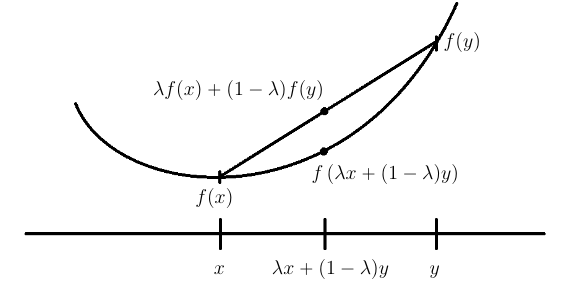
\includegraphics[scale=0.4]{konvex.png}
\end{center}
Wobei wir folgende Bemerkungen machen können:
\begin{enumerate}[(i)]
  \item Die Summe zweier konvexer Funktionen ist konvex
  \item $f$ ist genau dann konvex, falls für alle $x_0 < x < x_1$ in $\mathbf{I}$
  $$
    \frac{f(x) - f(x_0)}{x - x_0} \leq \frac{f(x_1) - f(x)}{x_1 - x_0}
  $$
  gilt.
  \item Sei $f: ]\,a, b\,[ \rightarrow \mathbf{R}$ in $]\,a, b\,[$ differenzierbar. Die Funktion
  $f$ ist genau dann (streng) konvex, falls $f'$ (streng) monoton wachsend ist. (z.B.: $f''(x) \geq 0$ ($f''(x) > 0$))
\end{enumerate}
% Höhere Ableitungen

\subsection{Höhere Ableitungen}

Sei $f: \mathbf{D} \rightarrow \mathbf{R}$ differenzierbar.
\begin{enumerate}[(i)]
  \item Für $n \geq 2$ ist $f$ $n$-mal differenzierbar in $\mathbf{D}$
  falls $f^{(n-1)}$ in $\mathbf{D}$ differenzierbar ist. Dann ist $f^{(n)} := (f^{(n-1)})'$
  und nennt sich die $n$-te Ableitung von $f$. Wobei zu beachten ist, dass: $n$-mal differenzierbar $\Rightarrow$ $(n-1)$-mal stetig differenzierbar.
  \item Die Funktion $f$ ist $n$-mal \textbf{stetig Differenzierbar}, falls sie $n$-mal
  differenzierbar ist und $f^{(n)}$ stetig ist. Wir definieren weiter die Menge $$C^n(\mathbf{D}) = \{f: \mathbf{D} \rightarrow \mathbf{R} \;|\; f\;n\text{-mal stetig diff'bar}\}$$
  \item Die Funktion $f$ ist in $\mathbf{D}$ \textbf{glatt} falls sie $\forall n \geq 1$ $n$-mal differenzierbar ist.
  $$C^\infty(\mathbf{D}) = \{f: \mathbf{D} \rightarrow \mathbf{R} \;|\; f\;\text{glatt}\}$$
\end{enumerate}
% Rechenregeln höherer Ableitungen

\subsection{Rechenregeln höherer Ableitungen}

Seien $f, g: \mathbf{D} \rightarrow \mathbf{R}$ $n$-mal differenzierbar:
\begin{enumerate}[(i)]
  \item $(f + g)^{(n)} = f^{(n)} + g^{(n)}$
  \item $(f * g)^{(n)} = \sum_{k = 0}^{n} \begin{pmatrix}
    n\\
    k
  \end{pmatrix} f^{(k)} * g^{(n - k)}$
  \item $\frac{f}{g}$ ist $n$-mal differenzierbar falls $g(x) \neq 0 \;\;\; \forall x \in \mathbf{D}$
  \item $(g \circ f)$ ist $n$-mal differenzierbar
  \item $e^x$, $sin(x)$ und $cos(x)$ sind glatte Funktionen
  \item Alle Polynome sind glatte Funktion
\end{enumerate}
% Taylor Approximation

\subsection{Taylor Approximation}

Sei $f: [\, a, b\,] \rightarrow \mathbf{R}$ stetig und in $]\, a, b\,[$
$(n+1)$-mal differenzierbar. Für jedes $a < x \leq b$ gibt es $\xi \in ]\,a, x\,[$ mit:
$$
f(x) = \sum_{k = 0}^n \frac{f^{(k)}(a)}{k!} * (x - a)^k + \frac{f^{(n + 1)}(\xi)}{(n + 1)!} * (x - a)^{n + 1}
$$
Man bemerke: der letzte Term $\frac{f^{(n + 1)}(\xi)}{(n + 1)!} * (x - a)^{n + 1}$ wird meist zur Fehlerabschätzung innerhalb eines Bereichs von $a$ verwendet.
Als Beispiel betrachte man $p(x) = x^3 + x + 1$ an der Stelle $a = 1$. Hier ist
die Taylor Approximation $$T_3 = 3 + 4(x - 1) + \frac{6}{2!}(x-1)^2 + \frac{6}{3!}(x-1)^3 = p(x)$$
und der Fehler für $\xi \in ]\,0, 2\,[$
$$
  |\text{Fehler}| \leq \frac{f^{(4)}(\xi)}{(4)!} * (x - 1)^{4} \leq \frac{0}{(4)!} * (1)^{4} = 0\\
$$
Ein weiteres Beispiel: Approximiere $\sqrt{9.2}$ mit einen Taylor Polynom
zweiten Grades.
\begin{align*}
  f(x) &= \sqrt{x}\\
  f'(x) &= \frac{1}{2} * x^{-0.5}\\
  f''(x) &= - \frac{1}{4} * x^{-1.5}\\
  f'''(x) &= \frac{3}{8} * x^{-2.5}\\
  T_2 f(x) &= f(x_0) + f'(x_0) * (x - x_0) + f''(x_0) * (x - x_0)^2\\
  R &= \frac{f'''(\xi)}{3!} * (x - x_0)^3 \text{ für $\xi \in (9, 9.2)$}\\
  &\Rightarrow x_0 = 9, \xi = 9\\
\end{align*}
% Sattelpunkt/ Horiz. Wendepunkt

\subsection{Sattelpunkt/ Horiz. Wendepunkt}

Ein Graphenpunkt wo $f'(x_0) = 0$, $x_0$ aber kein Extrema ist.
% Wendepunkt

\subsection{Wendepunkt}

Ein Wendepunkt ist ein Graphenpunkt wo der Drehsinn der Tangente sich ändert (In einem Wendepunkt gilt: $f''(x_0) = 0$)
% Spezielle Punkte bestimmen

\subsection{Spezielle Punkte bestimmen}

Sei $n \geq 0$, $a < x_0 < b$ und $f: [\,a, b\,] \rightarrow \mathbf{R}$ in $]\,a, b\,[$ $(n+1)$-mal stetig differenzierbar.
Annahme: $f'(x_0) = f''(x_0) = \cdots = f^{(n)}(x_0) = 0$
\begin{enumerate}[(i)]
  \item Falls $n$ gerade ist und $x_0$ eine lokale Extremalstelle, folgt $f^{(n+1)}(x_0) = 0$
  \item Falls $n$ ungerade ist und $f^{(n+1)}(x_0) > 0$ so ist $x_0$ eine strikte lokale Minimalstelle
  \item Falls $n$ ungerade ist und $f^{(n+1)}(x_0) < 0$ so ist $x_0$ eine strikte lokale Maximalstelle
\end{enumerate}
Ist $x_0$ jedoch keine Extremalstelle ($(i)$ von oben nicht erfüllt) bleiben zwei Optionen:
\begin{enumerate}[(i)]
  \item $f'(x_0) = 0 \land x_0 \text{ keine Extremalstelle} \Rightarrow x_0$ ist ein Sattelpunkt
  \item $f''(x_0) = 0 \land x_0 \text{ keine Extremalstelle} \Rightarrow x_0$ ist ein Wendepunkt
\end{enumerate}
% Integrale Ableiten

\subsection{Integrale Ableiten}

Hier ein Beispiel für die Ableitung eines Integrals:
\begin{align*}
  f(x) = -\int_2^{x^2} e^{-t^2} dt\\
  h(x) = e^{-t^2}\\
  \Rightarrow f(x) = - H(x^2) + H(2)\\
  \Rightarrow f'(x) = - h(x^2) 2x = -e^{-x^4} 2x
\end{align*}
\section{Integrieren}
\hypertarget{sec:4}{}
% Partition

\subsection{Partition}

Eine Zerlegung eines Intervalls $I = [\,a, b\,]$. Ist eine endliche Teilmenge
$P = \{a = x_0,\, x_1,\, \cdots,\, x_n = b\} \subset I$ wobei $x_0 < x_1 < \cdots < x_n$ und $\{a,\, b\} \subset P$
\\
Man bemerke: eine Partition $P'$ ist eine verfeinerung von $P$ falls $P \subset P'$
% Feinheit einer Partition

\subsection{Feinheit einer Partition}

Die \textbf{Feinheit} der Partition ist definiert durch $\delta(P) := \max_{1 \leq i \leq n} \delta_i = \max_{1 \leq i \leq n} (x_i - x_{i - 1})$
% Riehmannsche Summe

\subsection{Riehmannsche Summe}

Sei $\xi_i \in I_i$ zwischen Punkten. Jede Summe der Form
$$
  S(f, P, \xi) := \sum_{i = 1}^n f(\xi_i) * (x_i - x_{i - 1}) = \sum_{i = 1}^n f(\xi_i) * \delta_i
$$
nennt man eine \textbf{Riehmannsche Summe} der Partition $P$ und den Zwischenpunkten $\xi = \{\xi_1,\, \cdots,\, \xi_n\}$
% Unter-/ Obersumme

\subsection{Unter-/ Obersumme}

Wir definieren die Untersumme
$$
  s(f, P) := \sum_{i = 1}^n (\inf_{x \in I_i} f(x)) * \delta_i
$$
und die Obersumme
$$
  S(f, P) := \sum_{i = 1}^n (\sup_{x \in I_i} f(x)) * \delta_i
$$
% Eigenschaften der Unter-/ Obersumme

\subsection{Eigenschaften der Unter-/ Obersumme}

Sei $f: [a,\, b] \rightarrow \mathbf{R}$ eine beschränkte Funktion, sowie $P,\, Q \in P(I)$.
\begin{enumerate}[(i)]
  \item $P \subset Q \Rightarrow s(f, P) \leq s(f, Q) \leq S(f, Q) \leq S(f, P)$
  \item $\sup_{P \in \mathcal{P}(I)} s(f, P) \leq \inf_{Q \in \mathcal{P}(I)} S(f, Q)$
\end{enumerate}
% (Riehmann) Integrierbar

\subsection{(Riehmann) Integrierbar}

Sei $f:[a,\,b] \rightarrow \mathbf{R}$ beschränkt. Wir definieren zuerst $s(f) := \sup_{P \in \mathcal{P}(I)} s(f, P)$ sowie analog $S(f) := \inf_{P \in \mathcal{P}(I)} S(f, P)$.\\
Gilt
$$
  s(f) = S(f)
$$
so ist die $f$ Riehmann-Integrierbar und wird mit $\int_a^b f(x)dx$ bezeichnet.\\
Weiter sind folgende Aussagen äquivalent:
\begin{enumerate}[(i)]
  \item $f:[a,\, b]\rightarrow \mathbf{R}$ ist integrierbar mit $A := \int_a^b f(x) dx$
  \item $\forall \epsilon > 0 \;\;\; \exists P \in \mathcal{P}(I) \text{ mit } S(f, P) - s(f, P) < \epsilon$
  \item $\forall \epsilon > 0 \; \exists \delta > 0 \text{ so dass für jede Partition } P \in \mathcal{P}(I) $ mit $ \delta(P) < \delta $ und $ \xi_1, \cdots, \xi_n $ Zwischenpunkten $x_{k-1} \leq \xi_k \leq x_k:\;\;\; |A - S(f, P, \xi)| < \epsilon$
  \item Der Grenzwert $\lim_{\delta(P) \rightarrow 0} S(f, P, \xi) = \int_a^b f(x)dx$ existiert
\end{enumerate}
% Integrierbarkeit schnell zeigen

\subsection{Integrierbarkeit schnell zeigen}

Es gilt weiter für $f,g:[a,\,b] \rightarrow \mathbf{R}$ beschränkt, integrierbar und $\lambda \in \mathbf{R}$:
\begin{enumerate}[(i)]
  \item $f$ stetig $\Rightarrow f$ Integrierbar
  \item $f\text{ ist monoton} \Rightarrow f \text{ ist integrierbar}$
  \item $f + g$, $\lambda * f$, $f * g$, $|f|$, $max(f, g)$, $min(f, g)$ sind integrierbar sowie auch $\frac{f}{g}$ falls $|g(x)| \geq \beta > 0 \;\;\; \forall x \in [a,\,b]$
  \item Jedes Polynom auf $[a,\, b]$ ist integrierbar, auch $\frac{P(x)}{Q(x)}$ falls $Q(x)$ keine Nullstelle besitzt.
\end{enumerate}
% Majoranten Kriterium

\subsection{Majoranten Kriterium}

\begin{enumerate}[(i)]
  \item Falls $|f(x)| \leq g(x) \;\;\; \forall x \geq a$ und $g(x)$ auf $[a,\,\infty[$ integrierbar ist, so ist $f$ auf $[a,\,\infty[$ integrierbar.
  \item Falls $0 \leq g(x) \leq f(x)$ und $\int_a^\infty g(x) dx$ divergiert, so divergiert auch $\int_a^\infty f(x) dx$
  \item Sei $f:[1, \infty[ \rightarrow [0, \infty[$ monoton fallend. Dann konvergiert $\sum_{k = 1}^\infty f(k)$ genau dann, wenn $\int_1^\infty f(x) dx$ konvergent und in diesem
  Fall gilt: $0 \leq \sum_{k = 1}^\infty f(k) - \int_1^\infty f(x) dx \leq f(1)$
\end{enumerate}
% Rechenregeln für Integrale

\subsection{Rechenregeln für Integrale}

Es gelten folgene Rechenregeln:
\begin{enumerate}[(i)]
  \item $\int_a^b f(x) dx + \int_b^c f(x) dx = \int_a^c f(x) dx $ für $a < b < c$ mit $f:[a,\,c] \rightarrow \mathbf{R}$ und auf $[a,\,b]$ sowie $[b,\,c]$ integrierbar
  \item $\int_a^b(\alpha * f_1(x) + \beta * f_2(x)) dx = \alpha * \int_a^b f_1(x) dx + \beta * \int_a^b f_2(x) dx$ für $f_1$, $f_2: I \subseteq \mathbf{R} \rightarrow \mathbf{R}$ beschränkt Integrierbar mit endpunkten $a, b$ sowie $\alpha, \beta \in \mathbf{R}$
\end{enumerate}
% Abschätzungen von Integralen

\subsection{Abschätzungen von Integralen}

Es gibt folgende Absätzungen:
\begin{enumerate}[(i)]
  \item Seien $f, g: [a,\,b] \rightarrow \mathbf{R}$ beschränkt und integrierbar und $f(x) \leq g(x)\;\;\; \forall x \in [a,\,b]$. Dann folgt $\int_a^b f(x) dx \leq \int_a^b g(x) dx$
  \item Falls $f:[a,\,b] \rightarrow \mathbf{R}$ beschränkt und integrierbar folgt $|\int_a^b f(x) dx| \leq \int_a^b |f(x)| dx$
  \item $|\int_a^b f(x)g(x) dx| \leq \sqrt{\int_a^b f^2(x)} * \sqrt{\int_a^b g^2(x)}$
\end{enumerate}
% Mittelwertsatz der Integralrechnung

\subsection{Mittelwertsatz der Integralrechnung}

Seien $f,g:[a,\,b] \rightarrow \mathbf{R}$ wobei $f$ stetig und $g$ beschränkt integrierbar mit $g(x) \geq 0 \;\;\; \forall x \in [a,\,b]$ ist.
Dann gibt es $c \in [a,\,b]$ mit $$\int_a^b f(x) * g(x) dx = f(c) * \int_a^b g(x) dx$$
und falls $g \equiv 1$ erhalten wir $$\int_a^b f(x) dx = f(c) * (b - a)$$
% Stammfunktion

\subsection{Stammfunktion}

Sei $a < b$, $f:[a,\,b] \rightarrow \mathbf{R}$ stetig. Eine Funktion $F:[a,\,b] \rightarrow \mathbf{R}$ heisst
\textbf{Stammfunktion} von $f$ falls $F$ stetig differenzierbar in $[a,\, b]$ ist und $F' = f$ in $[a,\,b]$ gilt.
% Fundamentalsatz der Analysis

\subsection{Fundamentalsatz der Analysis}

Sei $f:[a,\,b] \rightarrow \mathbf{R}$ stetig. Dann gibt es eine Stammfunktion $F$ von $f$, die bis auf eine additive Konstante eindeutig bestimmt ist und es gilt:
$$\int_a^b f(x) dx = F(b) - f(a)$$

% Partielle Integration

\subsection{Partielle Integration}

Seien $a < b$ reele Zahlen und $f,g:[a,\,b] \rightarrow \mathbf{R}$ stetig differenzierbar.
Dann gilt:
$$
  \int_a^b f(x) * g'(x) dx = f(x) * g(x) \Big|_a^b - \int_a^b f'(x) * g(x) dx
$$
beziehungsweise für unbestimmte Integrale
$$
\int f(x) * g'(x) dx = f(x) * g(x) - \int f'(x) * g(x) dx
$$

\begin{itemize}
\item Polynome ableiten, wiederholende Fuktionen ($sin(x), cos(x), e^x$) integrieren
\item manchmal mit 1 multiplizieren
\end{itemize}
% Methode der Substitution

\subsection{Methode der Substitution}

Die Methode der Substitution ist die Umkehrung der Kettenregel. Sei $a < b$, $\phi:[a,\,b] \rightarrow \mathbf{R}$
stetig differenzierbar und $I \subset \mathbf{R}$ ein Intervall mit $\phi([a,\,b]) \subset I$ und $f: I \rightarrow \mathbf{R}$ eine stetige Funktion.
Dann ist
$$
  \int_a^b f(\phi(t)) * \phi'(t) dt = \int_{\phi(a)}^{\phi(b)} f(x) dx
$$
wobei für unbestimmte Integrale gilt:
$$
  \int f(\phi(t)) * \phi'(t) dt + C = \int f(x) dx \Big|_{x = \phi(t)}
$$
Hier ein Beispiel:
\begin{align*}
  \int 2x * cos(x^2) dx \Rightarrow u = x^2, \frac{du}{dx} = 2x, dx = \frac{du}{2x}\\
  = \int 2x * cos(u) * \frac{du}{2x} = \int cos(u) du = sin(x^2) + C\\
\end{align*}
% Integration konvergenter Reihen

\subsection{Integration konvergenter Reihen}

Sei $f_n:[a,\,b] \rightarrow \mathbf{R}$ eine Folge von beschränkten integrierbaren
Funktionen die gleichmässig gegen eine Funktion $f:[a,\,b] \rightarrow \mathbf{R}$ konvergiert.
Dann ist $f$ beschränkt, integrierbar und
$$
  \lim_{n \rightarrow \infty} \int_a^b f_n(x) dx = \int_a^b \lim_{n \rightarrow \infty} f_n(x) dx = \int_a^b f(x) dx
$$
Es gilt weiter: Sei $f_n:[a,\,b] \rightarrow \mathbf{R}$ eine Folge beschränkter und integrierbarer Funktionen so dass $\sum_{n = 0}^\infty f_n$ auf $[a,\,b]$
gleichmässig konvergiert. Dann gilt
$$
  \sum_{n = 0}^\infty \int_a^b f_n(x) dx = \int_a^b \sum_{n = 0}^\infty f_n(x) dx
$$
Es gilt weiter: Sei $f(x) := \sum c_k x^k$ eine Potenzreihe mit positiven Konvergenzradius $\rho > 0$.
Dann ist für jedes $0 \leq r < \rho$ $f$ auf $[-r,\,r]$ integrierbar und es gilt $\forall x \in ]-\rho,\,\rho[$
$$
  \int_0^x f(t) dt = \sum_{k = 0}^\infty \frac{c_k}{k+1} x^{k+1}
$$
% Stirlings Estimate
%
%\subsection{Stirlings Estimate};
%
%$$n! = \sqrt{2\pi n} (\frac{n}{e})^n exp(\frac{1}{12n} + R_3(n)) $$
% Uneigentliche Integrale

\subsection{Uneigentliche Integrale}

Sei $f:[a,\,\infty[ \rightarrow \mathbf{R}$ beschränkt und integrierbar auf $[a,\,b]$ für alle $b > a$. Wir definieren
$$
  \lim_{b \rightarrow \infty} \int_a^b f(x) dx = \int_a^\infty f(x) dx
$$
falls existent und sagen dass $f$ auf $[a, \infty[$ integrierbar ist.\\
Analog: Sei $f$ eine Funktion auf jedem Intervall $[a+\epsilon,\,b]\;\;\;\forall \epsilon > 0$
beschränkt und integrierbar. $f:]a,\,b] \rightarrow \mathbf{R}$ ist integrierbar falls der Folgende Grenzwert existiert, welchen wir als
$$
  \lim_{\epsilon \rightarrow 0+} \int_{a + \epsilon}^b f(x) dx := \int_a^b f(x) dx
$$
definieren. (Gilt auch symmetrisch für $[a,\,b-\epsilon]\;\;\;\forall \epsilon > 0$)
Wobei wir anmerken, dass $$\int_{-\infty}^\infty f(x) dx := \int_{-\infty}^c f(x) dx + \int_c^\infty f(x) dx$$
\\
% Partialbruchzerlegung

\subsection{Partialbruchzerlegung}

Seien $P, Q$ Polynome mit $grad(P) < grad(Q)$ und $Q$ mit der Produktzerlegung $Q(x) = \prod_{j = 1}^l \big( (x- \alpha_j)^2 + \beta_j^2\big)^{m_j} \prod_{i = 1}^k (x - \gamma_i)^{n_i}$. Dann gibt es $A_{ij}, B_{ij}, C_{ij}$ reelle Zahlen mit
$$
  \frac{P(x)}{Q(x)} = \sum_{i = 1}^l \sum_{j = 1}^{m_i} \frac{(A_{ij} + B_{ij}x)}{\big( (x- \alpha_i)^2 + \beta_i^2\big)^j} + \sum_{i = 1}^k \sum_{j = 1}^{n_i} \frac{C_{ij}}{(x-\gamma_i)^j}
$$
Bei einer Partialbruchzerlegung geht man folgendermassen vor:
\begin{enumerate}[(i)]
  \item Sei $R(x) = \frac{P(x)}{Q(x)}$. Falls $grad(P) \geq grad(Q)$ wenden wir Polynomdivision an.
  \item $Q$ lässt sich nun als $Q(x) = \prod_{j = 1}^l \big( (x- \alpha_j)^2 + \beta_j^2\big)^{m_j} \prod_{i = 1}^k (x - \gamma_i)^{n_i}$ zerlegen. Das sind
  die Komplexen und reelen Nullstellen mit ihrer vielfachheit.
  \item Wir bilden nun die "hässliche" Summe von oben
  \item Wir bestimmen mithilfe von Koeffizientenvergleich (Nennerpolynom Multiplizieren) die unbekannten $A_{ij}, B_{ij}, C_{ij}$.
\end{enumerate}
Hier ein einfaches Beispiel:
\begin{align*}
  &\frac{5x + 1}{x^2 + x - 2} = \frac{5x + 1}{(x - 1)(x + 2)} = \frac{A}{x - 1} + \frac{B}{x + 2} \\
  &\Rightarrow \text{ Löse } 5x + 1 = A(x + 2) + B(x - 1) \\
  &\Rightarrow \text{ Setze } x = -2,\;1
\end{align*}
Mit mehreren Linearen Faktoren:
\begin{align*}
  &\frac{-2x^2 + x + 8}{x (x-2)^2} = \frac{A}{x} + \frac{B}{x - 2} + \frac{C}{(x-2)^2} \\
  &\Rightarrow \text{ Löse } -2x^2 + x + 8 = A(x - 2)^2 + Bx(x - 2) + Cx
\end{align*}
Ohne reelle Nullstellen:
\begin{align*}
  &\frac{2x^2 -3x + 3}{(x-1)(x^2 + 1)} = \frac{A}{x - 1} + \frac{Bx + C}{x^2 + 1} \\
  &\Rightarrow \text{ Löse } 2x^2 -3x + 3 = A(x^2 + 1) + (Bx + C)(x - 1) \\
  &\Rightarrow \text{ Setze } x = 0,\;1,\;2
\end{align*}
% Unbestimmte Integral

\subsection{Unbestimmte Integral}

Das Unbestimmte Integral ist die Menge aller Stammfunktionen und sozusagen fast alles von oben gilt. $+C$ ist \textbf{sehr} wichtig.
\section{Sonstiges}
\subsection{Rewrite Function}
$h(x) = max{f(x), g(x)} = \frac{1}{2}(f(x) + g(x)) + \frac{1}{2}|f(x) -g(x)|$

\subsection{Proof of "Null-Reihe"}
Eine Reihe konvergiert, wenn die Folge ihrer Partialsumme $(s_n) n \in \mathbb{N} $ mit: $s_n = \sum_{i=1}^{n} a_i$ konvergiert, das heisst, es existiert ein Granzwert $s$, sodass
	$\lim_{n \to \infty} s_n = s$  Durch Umstellung der Reihe und mit den Rechenregeln für Grenzwerte gild dann
	$\lim_{n \to \infty} a_n = \lim_{n \to \infty} (s_n - s_{n - 1} = \lim_{n \to \infty} s_n - \lim_{n \to \infty} s_{n-1} =  s - s = 0$

\hypertarget{sec:5}{}
% Injektiv/ Surjektiv

\subsection{Injektiv/ Surjektiv}

Injektiv: $\forall a, b \in X, \;f(a) = f(b) \Rightarrow a = b$\\
\textit{$f$ ist injektiv Beweis: wenn Ableitung $>$ 0: dann streng monton wachsend auf ganz $\R$ und somit injektiv}\\
%TODO!!
Surjektiv: $\forall y \in Y, \, \exists x \in X, f(x) = y$
\textit{$f$ ist surjektiv Beweis: anhand von Zwischenwertsatz beweisen}\\
% Suprenum

\subsection{Suprenum}

Sei $A \subseteq \mathbf{R}$, $ A \neq \emptyset$ und $A$ nach oben beschränkt. Dann gibt es
eine kleinste obere Schranke von $A$. Es gibt also ein $c \in \mathbf{R}$ so dass:
\begin{enumerate}
  \item $\forall a \in A \; \; \; a \leq c$
  \item Falls $\forall a \in A \; \; \; a \leq x$ ist $c \leq x$
\end{enumerate}
Man bezeichnet $c := \sup A$ 
% Infimum

\subsection{Infimum}

Analog zum Suprenum die grösste untere Schranke.
% Dreiecksungleichung

\subsection{Dreiecksungleichung}

\begin{center}
  $\forall x, y \in \mathbf{R} : ||x| - |y|| \leq |x \pm y| \leq |x| + |y|$
\end{center}
% Bernoulli Ungleichung

\subsection{Bernoulli Ungleichung}

\begin{center}
  $ \forall x \in \mathbf{R} \geq -1$ und $n \in \mathbf{N}: (1 + x)^{n} \geq 1 + nx$
\end{center}
% Exponentialfunktion

\subsection{Exponentialfunktion}

Für ein $z \in \mathbf{C}$ berechnet man die Exponentialfunktion wie folgt:
$$
  exp(z) := 1 + z + \frac{z^2}{2!} + \cdots = \sum_{n = 0}^\infty \frac{z^n}{n!}
$$
und es gilt:
\begin{align*}
  exp(z) &= \lim_{n \rightarrow \infty} (1 + \frac{z}{n})^n
\end{align*}
Die reelle Exponentialfunktion $exp: \mathbf{R} \rightarrow ]0, \infty[$ ist streng monoton wachsend,
stetig und surjektiv.\\
Es gelten weiter folgende Rechenregeln:
\begin{enumerate}[(i)]
  \item $exp(x + y) = exp(x) * exp(y)$
  \item $x^a := exp(a * ln(x))$
  \item $x^0 = 1 \;\;\; \forall x \in \mathbf{R}$
  \item $exp(iz) = cos(z) + i*sin(z) \;\;\; \forall z \in \mathbf{C}$
  \item $exp(i*\frac{\pi}{2}) = i$
  \item $exp(i\pi) = -1$ und $exp(2\pi i) = 1$
  \item Für $a > 0$ ist $]0, +\infty[ \rightarrow ]0, +\infty[$ als $x \rightarrow x^a$ eine
  streng monoton wachsende stetige Bijektion
\end{enumerate}
Merke: $e^x$ entspricht $exp(x)$.
% Natürliche Logaritmus

\subsection{Natürliche Logaritmus}

Der natürliche Logaritmus wir als $ln: ]0, \infty[ \rightarrow \mathbf{R}$ bezeichnet
und ist eine streng monoton wachsende stetige funktion. Es gilt auch, dass
\begin{enumerate}[(i)]
  \item $ln(1) = 0$
  \item $ln(e) = 1$
  \item $ln(a * b) = ln(a) + ln(b)$
  \item $ln(a / b) = ln(a) - ln(b)$
  \item $ln(x^a) = a * ln(x)$
  \item $x^a * x^b = x^{a + b}$
  \item $(x^a)^b = x^{a * b}$
  \item $ln(1+x) = \sum_{n=1}^{\infty} \frac{(-1)^{n-1}}{n} x^n \;\;\; (-1 < x \leq 1)$
\end{enumerate}
% Faktorisierungs Lemma

\subsection{Faktorisierungs Lemma}

$$
  a^n - b^n = (a-b)(a^{n-1} + ba^{n-2} + \cdots + b^{n-2}a + b^{n-1})
$$
% Sinus Abschätzung

\subsection{Sinus Abschätzung}

Es gilt $|\sin(x)| \leq |x|$ mit folgendem Beweis:
\begin{align*}
  f(x) &= x - \sin(x), x \geq 0 \\
  f'(x) &= 1 - \cos(x) \geq 0
\end{align*}
Weil $f(0) = 0$, $f(x) \geq 0$ für $x > 0$. Dann $|\sin(x)| \leq |x|$ einfach. 
% Polynomiale Funktion

\subsection{Polynomiale Funktion}

Eine \textbf{Polynomiale Funktion} $P:\mathbf{R} \rightarrow \mathbf{R}$ ist eine Funktion
der Form $P(x) = a_nx^n + a_{n-1}x^{n-1} + \cdots + a_0$ wobei $a_0, a_1, \cdots, a_n \in \mathbf{R}$.
Falls $a_n \neq 0$, ist $n$ der Grad von $P$. 
% Kompaktes Intervall

\subsection{Kompaktes Intervall}

EIn Intervall $\subset \mathbf{R}$ ist kompakt, wenn es von der Form $\mathbf{I} = [a, b]$,
$a \leq b$ ist.
% Funktionenfolge

\subsection{Funktionenfolge}

Eine Funktionenfolge ist eine Abbildung:
\begin{align*}
  f:\mathbf{N} &\rightarrow \mathbf{R}^\mathbf{D} = \{f:\mathbf{D} \rightarrow \mathbf{R}\}\\
  n &\rightarrow f_n
\end{align*}
wobei $f_n: \mathbf{D} \rightarrow \mathbf{R}$ eine Funktion ist. Für jedes $x \in \mathbf{D}$
erhält man eine Folge $(f_n(x))_{n \geq 1}$ reeller Zahlen.
% Trigonometrische Funktionen

\subsection{Trigonometrische Funktionen}
Sind alle stetig
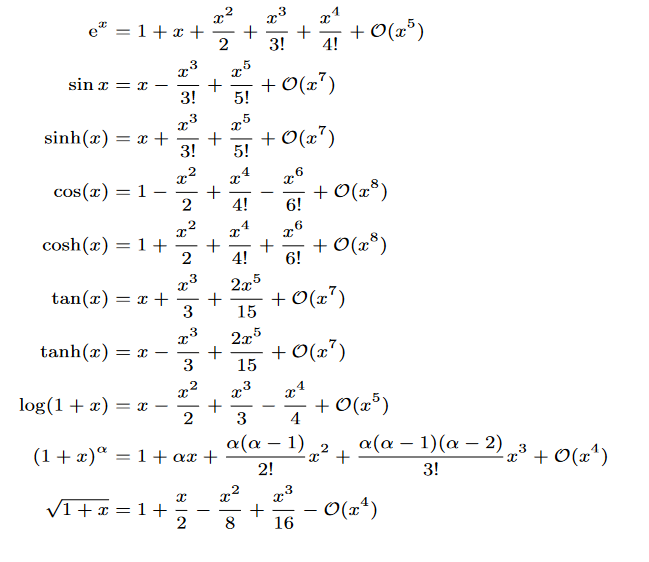
\includegraphics[width=6cm]{taylor.png}



\begin{enumerate}[(i)]
  \item $cos(z) = cos(-z)$
  \item $sin(-z) = -sin(z)$
  \item $cos^2(z) + sin^2(z) = 1 \;\;\; \forall z \in \mathbf{C}$
\end{enumerate}
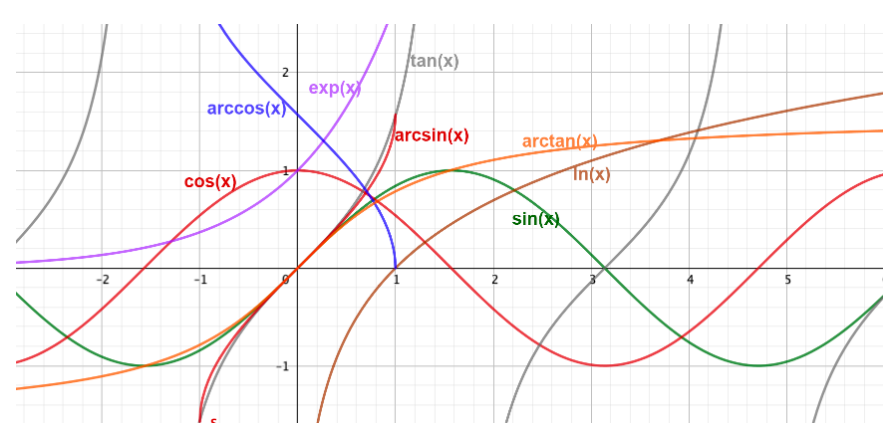
\includegraphics[width=7cm]{functions.png}
% Häufungspunkt

\subsection{Häufungspunkt}

$x_0 \in \mathbf{R}$ ist ein \textbf{Häufungspunkt} der Menge $\mathbf{D}$,
falls $\forall \delta > 0 \;\;\; (]x_0 - \delta, x_0 + \delta[ \setminus \{x_0\}) \cap \mathbf{D} \neq \emptyset$
% Lokales Extremum

\subsection{Lokales Extremum}

Eine Funktion $f$ besitzt ein lokales Extremum in $x_0$ falls es entweder ein lokales Minimum oder lokales Maximum von $f$ ist.
% Lokales Minimum

\subsection{Lokales Minimum}

Die Funktion $f$ besitzt ein lokales Minimum in $x_0$ falls es $\delta > 0$ gibt mit:
$$f(x) \geq f(x_0) \;\;\; \forall x \in ]x_0 - \delta, x_0 + \delta[\; \cap \; \mathbf{D}$$
% Lokales Maximum

\subsection{Lokales Maximum}

Die Funktion $f$ besitzt ein lokales Maximum in $x_0$ falls es $\delta > 0$ gibt mit:
$$f(x) \leq f(x_0) \;\;\; \forall x \in ]x_0 - \delta, x_0 + \delta[\; \cap \; \mathbf{D}$$
% Kritische Stelle

\subsection{Kritische Stelle}

Eine \textbf{kritische Stelle} einer Funktion ist ein $x_0$ an der $f'(x_0)$ null
oder undefiniert ist.
% Hyperbol Funktionen

\subsection{Hyperbol Funktionen}

\begin{enumerate}[(i)]
  \item $cosh(x) := \frac{e^x + e^{-x}}{2}: \mathbf{R} \rightarrow [1, \infty]$
  \item $sinh(x) := \frac{e^x - e^{-x}}{2}: \mathbf{R} \rightarrow \mathbf{R}$
  \item $tanh(x) := \frac{e^x - e^{-x}}{e^x + e^{-x}}: \mathbf{R} \rightarrow [-1, 1]$
\end{enumerate}
und es gilt $cosh^2(x) - sinh^2(x) = 1$



% Funktionen Verknüpfung
\subsection{Funktionen Verknüpfung}

$
x \mapsto (g \circ f)(x) := g(f(x))
$

\subsection{Sin/Cos Werte}
\begin{center}
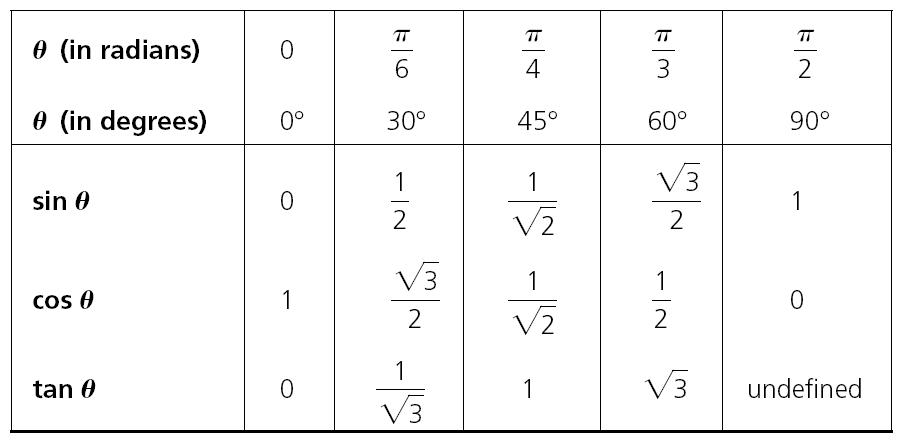
\includegraphics[scale=0.4]{values.png}
\end{center}


\section{Trigonometrie}

\subsection{Regeln}
\subsubsection{Periodizität}
\begin{itemize}
 \item $\sin(\alpha + 2 \pi) = \sin(\alpha) \quad \cos(\alpha + 2 \pi) = \cos(\alpha)$
 \item $\tan(\alpha + \pi) = \tan(\alpha) \quad \cot(\alpha + \pi) = \cot(\alpha)$
\end{itemize}

\subsubsection{Parität}
\begin{itemize}
 \item $\sin(-\alpha) = - \sin(\alpha) \quad \cos(-\alpha) = \cos(\alpha)$
 \item $\tan(-\alpha) = - \tan(\alpha) \quad \cot(-\alpha) = - \cot(\alpha)$
\end{itemize}

\subsubsection{Ergänzung}
\begin{itemize}
 \item $\sin(\pi - \alpha) = \sin(\alpha) \quad \cos(\pi - \alpha) = - \cos(\alpha)$
 \item $\tan(\pi - \alpha) = -\tan(\alpha) \quad \cot(\pi - \alpha) = - \cot(\alpha)$
\end{itemize}


\subsubsection{Komplemente}
\begin{itemize}
 \item $\sin(\pi/2 - \alpha) = \cos(\alpha) \quad \cos(\pi/2 - \alpha) = \sin(\alpha)$
 \item $\tan(\pi/2 - \alpha) = -\tan(\alpha) \quad \cot(\pi/2 - \alpha) = -\cot(\alpha)$
\end{itemize}

\subsubsection{Doppelwinkel}
\begin{itemize}
 \item $\sin(2\alpha) = 2 \sin(\alpha) \cos(\alpha)$
 \item $\cos(2\alpha) = \cos^2(\alpha) - \sin^2(\alpha) = 1 - 2 \sin^2(\alpha)$
 \item $\tan(2\alpha) = \frac{2\tan(\alpha)}{1 - \tan^2(\alpha)}$
\end{itemize}

\subsubsection{Addition}
\begin{itemize}
 \item $\sin(\alpha + \beta) = \sin(\alpha) \cos(\beta) + \cos(\alpha) \sin(\beta)$
 \item $\cos(\alpha + \beta) = \cos(\alpha) \cos(\beta) - \sin(\alpha) \sin(\beta)$
 \item $\tan(\alpha + \beta) = \frac{\tan(\alpha) + \tan(\beta)}{1 - \tan(\alpha) \tan(\beta)}$
\end{itemize}

\subsubsection{Subtraktion}
\begin{itemize}
 \item $\sin(\alpha - \beta) = \sin(\alpha) \cos(\beta) - \cos(\alpha)\sin(\beta)$
 \item $\cos(\alpha - \beta) = \cos(\alpha) \cos(\beta) + \sin(\alpha)\sin(\beta)$
 \item $\tan(\alpha - \beta) = \frac{\tan(\alpha) - \tan(\beta)}{1+\tan(\alpha) \tan(\beta)}$
\end{itemize}

\subsubsection{Multiplikation}
\begin{itemize}
 \item $\sin(\alpha) \sin(\beta) = -\frac{\cos(\alpha + \beta) - \cos(\alpha - \beta)}{2}$
 \item $\cos(\alpha) \cos(\beta) =  \frac{\cos(\alpha + \beta) + \cos(\alpha - \beta)}{2}$
 \item $\sin(\alpha) \cos(\beta) =  \frac{\sin(\alpha + \beta) + \sin(\alpha - \beta)}{2}$
\end{itemize}

\subsubsection{Potenzen}
\begin{itemize}
 \item $\sin^2(\alpha) = \frac{1}{2}(1-\cos(2\alpha))$
 \item $\cos^2(\alpha) = \frac{1}{2}(1+\cos(2\alpha))$
 \item $\tan^2(\alpha) = \frac{1-\cos(2\alpha)}{1+\cos(2\alpha)}$
\end{itemize}

\subsubsection{Diverse}

\begin{itemize}
 \item $\sin^2(\alpha) + \cos^2(\alpha) = 1$
 \item $\cosh^2(\alpha) - \sinh^2(\alpha) = 1$
 \item $\sin(z) = \frac{e^{iz} - e^{-iz}}{2}$ und $\cos(z) = \frac{e^{iz} + e^{-iz}}{2}$
\end{itemize}


\newpage

\section{Tabellen}
\subsection{Grenzwerte}
Wichtige Tabellen stehen hier
\begin{center}
  \begin{tabularx}{\linewidth}{XX}

    $\limxi \frac{1}{x} = 0$ & $\limxi 1 + \frac{1}{x} = 1$ \\
    $\limxi e^x = \infty$ & $\limxn e^x = 0$ \\
    $\limxi e^{-x} = 0$ & $\limxn e^{-x} = \infty$ \\
    $\limxi \frac{e^x}{x^m} = \infty$ & $\limxn xe^x = 0$ \\
    $\limxi \ln(x) = \infty$ & $\limxo \ln(x) = -\infty$ \\
    $\limxi (1+x)^{\frac{1}{x}} = 1$ & $\limxo (1+x)^{\frac{1}{x}} = e$ \\
    $\limxi (1+\frac{1}{x})^b = 1$ & $\limxi n^{\frac{1}{n}} = 1$ \\
    $\lim_{x\to\pm\infty} (1 + \frac{1}{x})^x = e$ & $\limxi (1-\frac{1}{x})^x = \frac{1}{e}$ \\
    $\lim_{x\to\pm\infty} (1 + \frac{k}{x})^{mx} = e^{km}$ & $\limxi (\frac{x}{x+k})^x = e^{-k}$ \\
    $\limxo \frac{a^x -1}{x} = \ln(a), \newline \forall a > 0$ &
    $\limxi x^a q^x = 0, \newline \forall 0 \le q < 1$ \\
  \end{tabularx}
  \begin{tabularx}{\linewidth}{XX}
    $\limxo \frac{\sin x}{x} = 1$ & $\limxo \frac{\sin kx}{x} = k$\\
    $\limxo \frac{1}{\cos x} = 1$ & $\limxo \frac{\cos x -1}{x} = 0$ \\
    $\limxo \frac{\log 1 - x}{x} = -1$ & $\limxo x \log x = 0$\\
    $\limxo \frac{1 - \cos x}{x^2} = \frac{1}{2}$ & $\limxo \frac{e^x-1}{x} = 1$ \\
    $\limxo \frac{x}{\arctan x} = 1$ & $\limxi \arctan x = \frac{\pi}{2}$ \\
    $\limxo \frac{e^{ax}-1}{x} = a$ & $\limxo \frac{\ln(x+1)}{x} = 1$ \\
    $\lim_{x\to 1} \frac{\ln(x)}{x-1} = 1$ & $\limxi \frac{\log(x)}{x^a} = 0$ \\
    $\limxi \sqrt[x]{x} = 1$ & $\limxi \frac{2x}{2^x} = 0$ \\
   % \bottomrule
  \end{tabularx}
\end{center}

\subsection{Ableitungen}
Kurze Notiz am Rande, ein stationärer Punkt ist: \\
$x \in \R$ mit $f'(x) = 0$
\begin{center}
  % the c>{\centering\arraybackslash}X is a workaround to have a column fill up all space and still be centered
  \begin{tabularx}{\linewidth}{c>{\centering\arraybackslash}Xc}
  
  $\mathbf{F(x)}$ & $\mathbf{f(x)}$ & $\mathbf{f'(x)}$ \\
  %\midrule
  $\frac{x^{-a+1}}{-a+1}$ & $\frac{1}{x^a}$ & $\frac{a}{x^{a+1}}$ \\
  $\frac{x^{a+1}}{a+1}$ & $x^a \ (a \ne -1)$ & $a \cdot x^{a-1}$ \\
  $\frac{1}{k \ln(a)}a^{kx}$ & $a^{kx}$ & $ka^{kx} \ln(a)$ \\
  $\ln |x|$ & $\frac{1}{x}$ & $-\frac{1}{x^2}$ \\
  $\frac{2}{3}x^{3/2}$ & $\sqrt{x}$ & $\frac{1}{2\sqrt{x}}$\\
  $-\cos(x)$ & $\sin(x)$ & $\cos(x)$ \\
  $\sin(x)$ & $\cos(x)$ & $-\sin(x)$ \\
  $\frac{1}{2}(x-\frac{1}{2}\sin(2x))$ & $\sin^2(x)$ & $2 \sin(x)\cos(x)$ \\
  $\frac{1}{2}(x + \frac{1}{2}\sin(2x))$ & $\cos^2(x)$ & $-2\sin(x)\cos(x)$ \\
  \multirow{2}*{$-\ln|\cos(x)|$} & \multirow{2}*{$\tan(x)$} & $\frac{1}{\cos^2(x)}$  \\
  & & $1 + \tan^2(x)$ \\
  $\cosh(x)$ & $\sinh(x)$ & $\cosh(x)$ \\
  $\log(\cosh(x))$ & $\tanh(x)$ & $\frac{1}{\cosh^2(x)}$ \\
  $\ln | \sin(x)|$ & $\cot(x)$ & $-\frac{1}{\sin^2(x)}$ \\
  $\frac{1}{c} \cdot e^{cx}$ & $e^{cx}$ & $c \cdot e^{cx}$ \\
  $x(\ln |x| - 1)$ & $\ln |x|$ & $\frac{1}{x}$ \\
  $\frac{1}{2}(\ln(x))^2$ & $\frac{\ln(x)}{x}$ & $\frac{1 - \ln(x)}{x^2}$ \\
  $\frac{x}{\ln(a)} (\ln|x| -1)$ & $\log_a |x|$ & $\frac{1}{\ln(a)x}$ \\
  %\bottomrule
  \end{tabularx}
\end{center}

\subsection{Weitere Ableitungen}
\begin{center}
  \begin{tabularx}{\linewidth}{>{\centering\arraybackslash}X>{\centering\arraybackslash}X}
  
  $\mathbf{F(x)}$ & $\mathbf{f(x)}$ \\
  \midrule
  $\arcsin(x) / \arccos(x)$ & $\frac{1 / -1}{\sqrt{1 - x^2}}$ \\
  $\arctan(x)$ & $\frac{1}{1 + x^2}$ \\ 
  $x^x \ (x > 0)$ & $x^x \cdot (1 + \ln x)$ \\
$f(x)^{g(x)}$ & $e^{g(x) ln(f(x))}$\\
$f(x) = cos(\alpha)$ & $f(x)^n = sin(x + n\frac{\pi}{2})$\\
$f(x) = \frac{1}{ax + b}$ & $f(x)^n = (-1)^n * a^n * n! * (ax + b)^{-n+1}$\\

  \bottomrule
  \end{tabularx}
\end{center}
\subsection{Integrale}
\begin{center}
 \begin{tabularx}{\linewidth}{>{\centering\arraybackslash}X>{\centering\arraybackslash}X}
  
  $\mathbf{f(x)}$ & $\mathbf{F(x)}$ \\
  \midrule
  $\int f'(x) f(x) \dx$ & $\frac{1}{2}(f(x))^2$ \\
  $\int \frac{f'(x)}{f(x)} \dx$ & $\ln|f(x)|$ \\
  $\int_{-\infty}^\infty e^{-x^2} \dx$ & $\sqrt{\pi}$ \\
  $\int (ax+b)^n \dx$ & $\frac{1}{a(n+1)}(ax+b)^{n+1}$ \\
  $\int x(ax+b)^n \dx$ & $\frac{(ax+b)^{n+2}}{(n+2)a^2} - \frac{b(ax+b)^{n+1}}{(n+1)a^2}$ \\
  $\int (ax^p+b)^n x^{p-1} \dx$ & $\frac{(ax^p+b)^{n+1}}{ap(n+1)}$ \\
  $\int (ax^p + b)^{-1} x^{p-1} \dx$ & $\frac{1}{ap} \ln |ax^p + b|$ \\
  $\int \frac{ax+b}{cx+d} \dx$ & $\frac{ax}{c} - \frac{ad-bc}{c^2} \ln |cx +d|$ \\
  $\int \frac{1}{x^2+a^2} \dx$ & $\frac{1}{a} \arctan \frac{x}{a}$ \\
  $\int \frac{1}{x^2 - a^2} \dx$ & $\frac{1}{2a} \ln\left| \frac{x-a}{x+a} \right|$ \\
  $\int \sqrt{a^2+x^2} \dx $ & $\frac{x}{2}f(x) + \frac{a^2}{2}\ln(x+f(x))$ \\
  \bottomrule
 \end{tabularx}
\end{center}



\end{multicols*}
\end{document}